\paragraph{Detalii implementare}
\begin{itemize}
\item
	\tab Proiectul facut se bazeaza pe comunicarea dintre cele 2 placi , Mega si Uno. Folosind modulul de comunicare i2c descris la inceput se realizeaza o conexiune master-slave intre cele 2 placi, master fiind MEGA, cu toata logica din spate, iar UNO find slave executand comenzi primite de la MEGA.\\
	\tab Diagrama de flowchart este urmatoarea.\\
	\begin{center}
	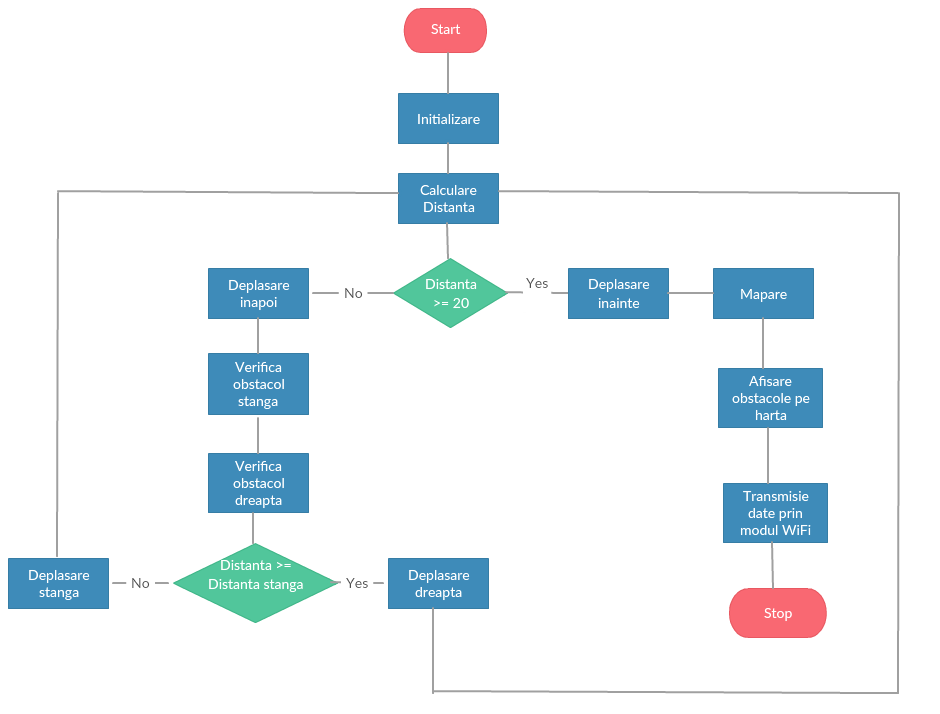
\includegraphics[scale=0.5]{flow.png}\\
	\end{center}
	\tab\tab \bf{Prima parte - modulul "slave" UNO)}\\
	\tab Uno contine codul pentru a rula motoarele servo si cele pentru roti. Motorul servo este folosit pentru a misca cu precizie un sonar ce este instalat peste el. Acest sonar citeste distantele folosind unde pe care le transmite si le receptioneaza, exact cum functioneaza si un liliac, si, din diferenta de timp dintre transmisie si receptia undei, se va calcula distanta din fata lui. Codul de miscare pentru servo este urmatorul.\\
	\begin{verbatim}
#include <Servo.h>
\\global Servo srv;
\\ in setup 
		void servo_move(int val)
{
   Serial.println(val);
  srv.attach(servoNumber);
  srv.write(val);
  delay(100);
  srv.detach();
  //Serial.println("Servo: ");
  //Serial.println(val);
 // delay(1000);
}
	\end{verbatim}
	\tab Se foloseste servo.attach pentru a porni motorul servo, mai mut ca si un enable,servoNumber). Mai apoi srv.write() va scrie gradul la care se va invarti servo(de la 0 la 360, 90 fiind in fata). Iar apoi se foloseste servo.detach() pentru a inceta transmisiunea.\\

	\tab Motoarele de la roti sunt actionate de 4 pini analogici(fiecare ptr un motor), avand capabilitatea PWD, adica sa reglam tensiunea transmisa lor astfel dand mai multa putere sau mai putin motorului. In setup, mai avem si definita comunicarea i2c, avand libraria Wire in care folosim Wire.begin(adresa), adresa unde se va conecta Mega.\\

	\begin{verbatim}
		void setup() {

 // Pornim busul I2C ca si slave la adresa 9
 Serial.begin(9600);
  pinMode(trigger, OUTPUT);
  pinMode(echo, INPUT);

  digitalWrite(mpin00, 0);
  digitalWrite(mpin01, 0);
  digitalWrite(mpin10, 0);
  digitalWrite(mpin11, 0);
 
  pinMode (mpin00, OUTPUT);
  pinMode (mpin01, OUTPUT);
  pinMode (mpin10, OUTPUT);
  pinMode (mpin11, OUTPUT);
 
  // pin LED
  pinMode(13, OUTPUT);


 Wire.begin(9);
 // Atasam o functie care sa se declanseze atunci cand primim ceva
 Wire.onReceive(receiveEvent);
 Serial.println("slave");
}

	/ Functie pentru controlul unui motor
// Intrare: pinii m1 si m2, directia si viteza
void StartMotor (int m1, int m2, int forward, int speed)
{
   
  if (speed==0) // oprire
  {
    digitalWrite(m1, 0);
    digitalWrite(m2, 0);
  }
  else
  {
    if (forward)
    {
       digitalWrite(m2, 0);
       analogWrite (m1, speed); // folosire PWM
    }
    else
    {
      digitalWrite(m1, 0);
      analogWrite(m2, speed);
  }
 }
 srv.write(90);
}
	\end{verbatim}

	\tab Functiile pentru deplasarea motorului in fata, spate, stanga ,dreapta sunt urmatoarele, si se bazeaza pe actionarea simultana a motoarelor, sau doar cate unu.\\

	\begin{verbatim}
		void move_down(){
  
    StartMotor (mpin00, mpin01, 1, 128);
    StartMotor (mpin10, mpin11, 1, 128);
    delay(400);
    delayStopped(100);
    

    //Serial.print("down");

}

void move_up(){
  
  StartMotor (mpin00, mpin01, 0, 128);
  StartMotor (mpin10, mpin11, 0, 128);
  delay(200);
  delayStopped(100);
  

  //Serial.print("up");
}

 
void move_left(){
  
  StartMotor (mpin00, mpin01, 0, 128);
  StartMotor (mpin10, mpin11, 1, 128);
  delay(400);
  delayStopped(300);
  

  //Serial.print("left");
}

 
void move_right(){
  
  StartMotor (mpin00, mpin01, 1, 128);
  StartMotor (mpin10, mpin11, 0, 128);
  delay(400);
  delayStopped(300);
  
  //Serial.print("right");
}
	\end{verbatim}

	\tab Functia de receptie a datelor transmise de Mega catre Uno. Se va folosi o coada in Uno ,pentru a stoca comenzile primite de Mega astfel : pana executa o comanda, el va memora celelalte primite si le va executa pe rand in ordine, fara sa piarda vreo comanda.\footnote{Libraria de queue.h este luata de pe site-ul de la arduino}.
	\begin{verbatim}
		// Atasam o functie care sa se declanseze atunci cand primim ceva
 		Wire.onReceive(receiveEvent); // in setup

	void receiveEvent(int bytes) {
	 x = Wire.read(); // citim un character din I2C
 	  queue.push(x);
	}
	\end{verbatim}
	\tab Logica placii UNO va fi urmatoarea: intr-un interval de timp sau dupa finalizarea ultimei comenzi se va scoate din coada urmatoarea comanda de executat si se va procesa de functia computeLogic care va stii sa miste motoarele in fata,spate,stanga,dreapta, ori servo in functie de ce ii dicteaza logica din MEGA.\\

	\begin{verbatim}
		void loop() {
 
  //Serial.println(x);
  //delay(300);
  //servo_move1();
   currentMillis = millis();
      if(currentMillis - previousMillis > interval){
        int c = queue.pop();
       // int c2 = queue.pop();
        //Serial.println(c);
        //(c !=0 && c2 != 0){
            computeLogic(c);
            Serial.print(c);
          //}
        //Serial.println(x);
        previousMillis = currentMillis;
         
      }
 
  //move_head_in_front();
}

void computeLogic(int x){
  switch(x) {
   case 1:
      move_down();
      break;
   case 2:
      move_up();
      break;
   case 3:
      move_left();
      break;
   case 4:
      move_right();
      break;
   case 6:
      srv.detach();
      break;
   case 7:
      srv.attach(servoNumber);
      break;
   case 8:
      delayStopped(300);
      break;
   default :
        servo_move(x);
      //Serial.println(x);
      //servo_move1();
      break;
  }
}
	\end{verbatim}
	\tab\tab \bf{A doua parte - modulul "master" MEGA}\\

	\tab "Creierul" robotului, Mega va primii semnale de la modului wi-fi, cat si de la sonar. Cu aceste date el va calcula distantele primite si  va genera o harta 2d in care mapeaza obiectele detectate si o transmite prim wi-fi catre pagina web a device-ului connectat la acesta.\\
	\begin{verbatim}
		void loop() {  
  int distanceRight = 0;
  int distanceLeft = 0;

   //citire();
   
 // logic_of_movement(distanceRight,distanceLeft);
  for(int i=0; i<10; i++){
     move_head_in_front();
     distanta();
     
     logic_of_movement(distanceRight,distanceLeft);
     citire();
     citire2();
  }
}
	\end{verbatim}

	\tab Functia logic-of-movement genereaza logica de miscare a robotului, verificand distanta primita ca sa nu se loveasca de vreun obiect, miscarea principala a robotului va fi in fata, si la fiecare cateva sute de milisecunde se va opri sa scaneze harta. Cand detecteaza obstacol in fata, se va da putin in spate si va alege pe udne sa mearga(stanga ,dreatpa).\\
	\begin{verbatim}
		void logic_of_movement(int distanceRight,int distanceLeft){
  if(distance >= 20){
      move_up();
      mapare();
  }
  else{
      delayStopped();
      move_down();
      distanceRight = checkRight();
      delay(100);
      distanceLeft = checkLeft();
      delay(100);

      if(distance >= distanceLeft){
          move_right();
          //delayStopped(300);
      }
      else{
          move_left();
          //delayStopped(300);
      }
  }
}
	\end{verbatim}

	\tab Functiile checkRight , checkLeft vor trimite comenzi la UNO pentru a verfica daca este un obiect in stanga sau in dreapta , prin msicarea motoarelor servo.Iar in logica va merge unde este distanta cea mai mare(nu este obiect langa).\\
	\begin{verbatim}
		
int checkRight(){
  move_servo(50);
  delay(500);
  distanta();
  delay(50);
  int dist = distance;
  delay(100);
  return dist;
}

int checkLeft(){
  move_servo(170);
  delay(500);
  distanta();
  delay(50);
  int dist = distance;
  delay(100);
  return dist;
}

	\end{verbatim}
		

	\tab Functia de mapare va scana intreg perimetrul ep o raza de 180 de grade din 20 in 20 si le va salva intr-o matrice de distante cu care se va calcula harta obiectelor .\\
	\begin{verbatim}
		void mapare(){
       //directie[0]=0;
       for(int j =0; j<=180; j+=20){
        nuTransmite = false;
        move_servo(j);
        delay(300);
        distanta();
        harta[i][j/20] = distance;
       }
       nuTransmite= true;
       if(i > 10){
        j = 0;
       }else{
        i++;
       }
       //delay(300);
}
	\end{verbatim}

	\tab Distanta este calculata folosind timpul micros(), trimitand o unda si asteptand sa o receptioneze , difernta de timp introdusa intr-o formula va da distanta.\footnote{idee preluata de pe site-ul arduino}.
	\begin{verbatim}
		void distanta(){
 
  digitalWrite(trigger,HIGH);
  delay(10);
  digitalWrite(trigger,LOW);
 
  while ( digitalRead(echo) == 0 );
  t1 = micros();
  while (digitalRead(echo) == 1);
  t2 = micros();
  pulse_width = t2 - t1;
  distance = pulse_width/58.0;
 
  if ( pulse_width > MAX_DIST ) {
    //distance = MAX_DIST/58.0;
   // Serial.println("Out of range");
  }
  else {
    //Serial.print(distance);
   // Serial.println("cm");
  }
  delay(10);
}
	\end{verbatim}

	\tab Functiile de msicare move-up, move-down, move-servo, vor deschide un canal de transmise cu Uno vor transmite comanda, iar apoi il vor inchide, toate functionand pe acelasi tipar.\\

	\begin{verbatim}
		void move_down(){
 
 Wire.beginTransmission(9); // transmitem spre device #9
 Wire.write(1); // trimitem x
 Wire.endTransmission(); // oprim transmisia

}
	\end{verbatim}

	\tab In setup se va initializa comunicarea i2c, modulul wi-fi cat si sonarul.\\

	\begin{verbatim}
		Serial.begin(115200); \\wifi
  Serial1.begin(115200);  \\wifi
  Wire.begin(); 	\\i2c
 
  pinMode(LED_BUILTIN, OUTPUT); 
  digitalWrite(LED_BUILTIN, LOW); 
  sendData("AT+RST\r\n", 2000, false); // resetare modul 
  sendData("AT+CWMODE=2\r\n", 1000, false); // configurare ca access point 
  sendData("AT+CIFSR\r\n", 1000, DEBUG); // citeste adresa IP 
  sendData("AT+CWSAP?\r\n", 2000, DEBUG); // citeste informatia SSID (nume retea) 
  sendData("AT+CIPMUX=1\r\n", 1000, false); // configurare conexiuni multiple 
  sendData("AT+CIPSERVER=1,80\r\n", 1000, false); // pornire server pe port 80 
  //Serial.println("master");
  pinMode(trigger, OUTPUT); \\sonar
  pinMode(echo, INPUT); \\sonar
	\end{verbatim}

	\tab Functia sendData este cea luata din laborator pentru a transmite comenzile din setup cat si textul ce il vrem afisat. Iar functia de citire va folosi sendData pentru a scrie pe browser harta obiectelor.\\
	\begin{verbatim}
		void citire2(){

   if (Serial1.available()) { 
    if (Serial1.find("+IPD,")) { 
      delay(500); 
      int connectionId = Serial1.read() - 48; // functia read() returneaza valori zecimale ASCII 
      // si caracterul ‘0’ are codul ASCII 48 
      String webpage = "<h1>Harta de vizualizare!</h1>"; 
      String cipSend = "AT+CIPSEND="; 
      cipSend += connectionId; 
      cipSend += ","; 

      //harta[0][0] = 39;
      //harta[0][1] = 40;
      //harta[1][0] = 41;
      //harta[1][1] = 42;
      for(int i=0; i<10; i++){
        webpage += "<p>";  \\transmite sub forma de paragraf, html
       for(int j=0; j<9; j++){
          if(harta[i][j] > 40){
            //Serial.print("_");
             //webpage += i; 
             // webpage += "  ";   
            // webpage += j;  
             webpage += "_";  
          }else{
             // webpage += i; 
             // webpage += "  ";   
            // webpage += j;  
             webpage += "X"; 
            //Serial.print("X");
          }
          //Serial.print(harta[i][j]);
           //webpage += harta[i][j];
            webpage += " ";  
          //Serial.print(" ");
       }
        webpage += "</p>"; 
      //Serial.println();
      } 

      cipSend += webpage.length();  \\la final trimitem lungimea cat si semnalul de comanda
      cipSend += "\r\n"; 
      sendData(cipSend, 100, DEBUG); 
      sendData(webpage, 150, DEBUG); 
      String closeCommand = "AT+CIPCLOSE="; 
      closeCommand += connectionId; //se adauga identificatorul conexiunii 
      closeCommand += "\r\n"; 
      sendData(closeCommand, 300, DEBUG); 
  }
 
  }
  
}
       \end{verbatim}
\end{itemize}
	